%====================================================================================================
% ?????
%====================================================================================================
% TCC
%----------------------------------------------------------------------------------------------------
% Autor				: Jasane Schio
% Orientador		: Gedson Faria
% Co-Orientador		: Angelo Darcy
% Instituição 		: UFMS - Universidade Federal do Mato Grosso do Sul
% Departamento		: CPCX - Sistema de Informação
%----------------------------------------------------------------------------------------------------
% Data de criação	: 01 de Outubro de 2015
%====================================================================================================

\documentclass[a4paper,12pt,brazil]{dct-class}
\usepackage[brazil]{babel}

\usepackage{algorithm, algpseudocode}
\renewcommand{\listalgorithmname}{Lista de Algoritmos}
\floatname{algorithm}{Algoritmo}
\algrenewcommand\algorithmicwhile{{\bf enquanto}}
\algrenewcommand\algorithmicdo{{\bf faça}}
\algrenewcommand\algorithmicif{{\bf se}}
\algrenewcommand\algorithmicelse{{\bf senão}}
\algrenewcommand\algorithmicend{{\bf fim}}
\algrenewcommand\algorithmicthen{{\bf então}}
\algrenewcommand\algorithmicfor{{\bf para}}
\algrenewcommand\algorithmicforall{{\bf para todo}}

\usepackage[utf8]{inputenc}
\usepackage[top=25mm,bottom=25mm,left=25mm,right=20mm]{geometry}
\usepackage{caption}
\usepackage{subcaption}
\usepackage{pdfpages}
\usepackage{abntex2cite}
\usepackage{setspace}
%\usepackage{caption}
\usepackage[font=small]{caption}

%\DeclareCaptionFormat{myformat}{#1#2#3\hrulefill}
%\captionsetup{format=myformat}
%\captionsetup[lstlisting]{position=bottom}
%\captionsetup[lstinputlisting]{position=bottom,format=myformat}
\usepackage{graphicx}
\usepackage{multicol}
\usepackage{indentfirst}
\usepackage{booktabs}	% http://ctan.org/pkg/booktabs
\usepackage{array}		% http://ctan.org/pkg/array
\newcolumntype{M}{>{\centering\arraybackslash}m{\dimexpr.25\linewidth-2\tabcolsep}}
\usepackage{listings}
\usepackage{color}

\begin{document}

\thispagestyle{empty}
\include{cabecalho}
%\include{resumo}
%\include{abstract}
%\include{agradecimentos}

\tableofcontents

%\printglossaries

\cleardoublepage
\phantomsection
\addcontentsline{toc}{chapter}{Lista de Figuras}
\listoffigures

%\cleardoublepage
%\phantomsection
%\addcontentsline{toc}{chapter}{Lista de Tabelas}
%\listoftables

%\cleardoublepage
%\phantomsection
%\addcontentsline{toc}{chapter}{Lista de Algoritmos}
%\listofalgorithmes

%\cleardoublepage
%\phantomsection
%\addcontentsline{toc}{chapter}{Lista de Quadros}
%\lstlistoflistings

% lista de abreviaturas e siglas
% o parametro deve ser a abreviatura mais longa
%\begin{listofabbrv}{SPMD}
%	\item[CMM] Capability Maturity Model
%	\item[SMP] Symmetric Multi-Processor
%	\item[NUMA] Non-Uniform Memory Access
%	\item[SIMD] Single Instruction Multiple Data
%	\item[SPMD] Single Program Multiple Data
%	\item[ABNT] Associação Brasileira de Normas Técnicas
%\end{listofabbrv}

%\pdfbookmark[0]{\lstlistlistingname}{lol}
%\begin{KeepFromToc}
%\lstlistoflistings
%\end{KeepFromToc}
%\cleardoublepage

\include{introducao} % Introdução
%====================================================================================================
% ?????
%====================================================================================================
% TCC
%----------------------------------------------------------------------------------------------------
% Autor				: Jasane Schio
% Orientador		: Gedson Faria
% Co-Orientador		: Angelo Darcy
% Instituição 		: UFMS - Universidade Federal do Mato Grosso do Sul
% Departamento		: CPCX - Sistema de Informação
%----------------------------------------------------------------------------------------------------
% Data de criação	: 01 de Outubro de 2015
%====================================================================================================
% Define o caminho das figuras
\graphicspath{{figuras/}}
\chapter{Fundamentação Teórica} \label{Cap:Fundamentacao}

%\section{Estado da Arte} \label{Sec:EstadoDaArte}
%Como estado da arte foram relacionados os métodos de detecção de objetos em imagens em tempo real e estáticas.

\section{Processamento de Imagens}
\subsection{Detecção de Objetos}
\label{Sec:TiposDeDeteccaoDeObjetos}
Antes de descrever os métodos de classificação devemos fazer algumas definições:
\begin{itemize}
	\item	Em cada detecção de objetos são obtidas as informações sobre a imagem, essas são de acordo com o tipo de detecção desejada. Os dados podem conter informações como posição, tamanho, borda, transformação linear, rotação entre outros. Cada detecção em uma imagem é chamada de pose.
	
	\item	Métodos de detecção de objeto baseado em classes constroem a classe do objeto baseada em um conjunto de treino. O conjunto de treino é composto por múltiplas imagens exemplo do objeto para que seja assim capturado os aspectos do objeto.
\end{itemize}

A detecção de objetos pode ser considerada uma técnica herdada do reconhecimento de padrões da área de aprendizado de máquina, esta consiste em separar objetos por categorias de acordo com uma ou mais características especificas. Quando essa técnica se junta ao processamento de imagens, onde são acentuadas as características especificas do objeto dentro da imagem para assim este se destacar, tornou-se possível a detecção de objetos em imagens que dentro do campo de visão computacional é uma das áreas que mais obtêm a atenção de pesquisadores. O primeiro Framework de métodos que usam base de dados categorizando uma ou mais características de um objetos para fazer o reconhecimento através de aprendizado foi apresentado em 2001 por Viola e Jones\cite{Viola:2001}. Desde o framework de Viola e Jones até os dias atuais muitos métodos e teorias para detecção já foram propostos e implementados como detecção de faces utilizando um classificador de redes neurais na intensidade de padrões de uma imagem, support vector machine para localizar rostos humanos e carros\cite{Nascimento:2007}, análise de componentes principais, análise independente de componentes, fatoração de matriz não-negativa, análise discriminativa linear, boosting\cite{Roth:2008}, além da classificação binaria, onde se considera a detecção do objeto em tamanho fixo apenas variando na posição na imagem\cite{AmitFelzenszwalb:2014}. 

Em 2005 Ulusoy e Bishop\cite{Ulusoy:2005} mostraram o quão útil seria categorizar os métodos de detecção de imagens, e os dividiram em duas principais categorias: generativa e discriminativa. Categorias que foram aceitas e utilizadas como mostram Amit e Falzenszwalb\cite{AmitFelzenszwalb:2014} e Roth e Winter\cite{Roth:2008}.

O método generativo pode ser descrito como um modelo probabilístico para a variância da pose de um objeto juntando com o modelo de aparência, ou seja, um modelo de probabilidade para a aparência da imagem condicional em uma determinada pose, juntamento com um modelo de fundo. Os parâmetros do modelo são estimados a partir de dados retirados de treinamento e as decisões são baseadas nas probabilidades anteriores\cite{AmitFelzenszwalb:2014}. Em resumo o método generativo tenta encontrar uma representação adequada dos dados originais através da aproximação dos dados originais, mas mantendo o máximo de informação possível\cite{Roth:2008}.

Já o modelo discriminativo tipicamente constrói um classificador que pode discriminar entre imagens (ou sub-imagens) contendo o objeto e as que não contém o objeto. Os parâmetros do classificador são selecionados para minimizar os erros nos dados de treino\cite{AmitFelzenszwalb:2014}.


%	Ulusoy\cite{Ulusoy:2005} apontou as principais vantagens dos dois metodos. 
Segundo Ulusoy e Bishop\cite{Ulusoy:2005} o método generativo se destaca por tratar perda de dados ou dados parcialmente rotulados, pela facilidade em que uma nova classe pode ser incrementada na classificação condicional de densidade, independentemente das classes anteriores, e por conseguir facilmente lidar com composição de objetos (ex: óculos, chapéus...), considerando que os modelos discriminativos precisar analisar todas as combinações durante o treinamento. Amit e Felzenszwalb\cite{AmitFelzenszwalb:2014} ainda aponta que as vantagens descritas sobre o método discriminativo são ditas como a flexibilidade do modelo  que pode ser utilizado em regiões do espaço de entrada onde as probabilidades posteriores diferem significativamente de 0 ou 1, ao passo que as abordagens detalhes generativas modelo de distribuição de X, que podem ser irrelevantes para determinar as probabilidades posteriores, além de ser tipicamente muito rápido em fazer previsões para os novos pontos (teste) de dados, enquanto os modelos generativos muitas vezes exigem solução iterativa, e pela igualdade de circunstâncias, seria de esperar que os métodos discriminativos tenham melhor desempenho preditivo, uma vez que são treinados para prever o rótulo de classe em vez de a distribuição conjunta de vetores e alvos de entrada.

\subsection{Detecção de Bordas}
Para um objeto poder ser detectado por algum método de detecção de objetos a imagem passa por um processo de segmentação. A segmentação pode ser dita como o processo de divisão da imagem em objetos\cite{Gonzalez:2008}. De acordo com Wangenheim\cite{Wangenheim:2014} o processo de segmentação se baseia em dois conceitos: similaridade e descontinuidade. A descontinuidade é o processo onde se separa o fundo das partículas e estas umas das outras, através de linhas, bordas ou pontos. Já a similaridade é o processo onde os pixeis provenientes da descontinuidade são agrupados de acordo com a proximidade um dos outros para formar os objetos de interesse. De acordo com Canny\cite{Canny:1986} o processo de detecção de bordas é um processo simplificado que serve para diminuir drasticamente o total de dados a serem processados e ao mesmo que o mesmo preserva informações valiosas sobre os objetos. É muito comum a ocorrência de ruídos quando se trata da detecção de bordas, e por sua vez para evitar esses ruídos é necessário a suavização da imagem antes de fazer a detecção. Vale\cite{Vale:2002} lembra que a suavização possui pontos negativos como perda de informação e deslocamento de estruturas de feições proeminentes no plano da imagem. Além disso, existem diferenças entre as propriedades dos operadores diferenciais comumente utilizados, o que ocasiona  bordas diferentes.Assim, como dito por Ziou e Tabbone citados por Vale\cite{Vale:2002}, se torna difícil encontrar um algoritmo que tenha bom desempenho em diferenciados contextos e capture os requisitos necessários aos estágios subsequentes do processamento. 
Quando se trata de detecção de bordas existem dois critérios\cite{Canny:1986} para essa detecção que devem ser levados em consideração, Taxa de Erro e Localização\cite{Vale:2002}. 
\begin{description}
	\item[Taxa de Erro] É importante que as bordam contidas na imagem não sejam confundidas ou perdidas e ainda que não sejam detectadas bordas falsas. É necessário que o algoritmo de detecção de borda tenha uma baixa taxa de erro para que seja eficiente.\cite{Wangenheim:2014, Canny:1986, Vale:2002}
	\item[Localização] A distância entre os pixels de borda encontradas pelo algoritmo e a borda atual deveriam ser o menor possível.\cite{Wangenheim:2014}
\end{description}
Ao tentar aplicas esses dois critérios para desenvolver um modelo matemático para detecção de bordas sem a necessidade de base em regras preestabelecidas em seu artigo
\textit{ A Computational Approach to Edge Detection} Canny percebeu que somente esses dois critérios não eram o suficiente para obter uma boa precisão da detecção de bordas. E então propôs um terceiro critério: Resposta.
\begin{description}
	\item[Resposta] Para contornar a possibilidade de mais de uma resposta para a mesma borda, ou seja o detector de bordas não deveria identificar múltiplos pixels de borda onde somente exista um único pixel. \cite{Wangenheim:2014, Canny:1986, Vale:2002}
\end{description}

Com o acréscimo do terceiro critério então nota-se que o processo de detecção de bordas de Canny
mostrou-se bastante flexível, independente da origem da imagem utilizada\cite{Vale:2002}.









\section{Cores} \label{Sec:Cores}


O olho humano é capaz de identificar cores mesmo com as mais diferentes interferências, luminosidade, tonalidade, intensidade, entre outras ações de agentes externos graças aos \textbf{cones} e \textbf{bastonetes}. Os bastonetes são os responsaveis por distinguirem tons de cinza e pela visão periferica e tem como caracteristica serem sensiveis a baixo nivel de luminosidade\cite{Azevedo:2003}, os cones, por sua vez, são sensiveis ao alto nivel de iluminação e responsaveis pela percepçao de cores\cite{Azevedo:2003}. A informação obtida por ambos é assimilada pelo nosso  cérebro, ligando a cor a sua aparência, já para uma máquina cores são números, códigos, cada cor contém um código especifico e cada uma de suas variâncias e alterações também. Para o nosso cérebro é muito fácil entender, exemplo, que o verde, verde lima, verde escuro são a mesma cor, apenas com tonalidades diferentes, já para o computador estas são: (0,255,0),(50,205,50),(0,128,0), no padrão de cor RGB que considera uma luz visível. Mas se for aplicado luminosidade nessas cores, por exemplo, elas ainda se tornam outras diferentes cores, um código diferente para cada luminosidade possível. Para conseguir cobrir todas essas alterações nas cores foram definidos em 1921 começaram então pela Comissão Internacional de Iluminação (CEI) a serem definidos espaços e modelos de cores\cite{Souto:2003}.

\subsection{Espaços de Cores}
Segundo Foley et. al citado por Souto\cite{Souto:2003} espaço de cores é um sistema tridimensional de
coordenadas, onde cada eixo refere-se a uma cor primária. A quantidade de cor primária
necessária para reproduzir uma determinada cor, é atribuída a um valor sobre o eixo
correspondente. O espaço de cores pode ser entendido como a quantidade de detalhamento, tonalidades de uma cor, dentro do espectro de cores de um determinado modelo de cor. 
Quando fez sua primeira experiência com a decomposição da luz em um prisma para obter cores Newton percebeu que não havia a cor branca. Ele tentou então misturar as sete cores que obteve para gerar a branca, sem sucesso. Parar gerar a cor branca é necessário a soma das três cores primarias azul, verde e vermelho. Apos anos de estudo entendeu-se que existe duas formas de se obter cores: através da emissão ou reflexão de luz, espaços RGB e CMY respectivamente, \figurename{ 2.2}. 

\subsubsection{RGB}
O espaço de cores que emitem luz é conhecido como RGB que é baseado na teoria das cores primarias vermelho, verde e azul, em inglês Red, Green, Blue, para simular a tricromática visão humana, onde toda cor é composta pela soma das três cores.
\subsubsection{CMY}
O espaço de cores que refletem luz é conhecido como CMY que são as cores ciano, magenta e amarelo, em inglês Cyan, Magenta e Yellow. Neste espaço a cor é obtida pela subtração das cores. Existe uma variação ao CMY chamada de CMYK onde é acrescentada a cor preta e foi criado 	como uma opção mais barata, pois não necessita de pigmentos puros\cite{Rocha:2010}.
\newline
\begin{figure}[!h]
	\centering
	\includegraphics[width=0.8\textwidth]{espacos.pdf}
	\caption{Exemplo dos espaços de cores RGB E CMY.}
	\label{Espaco de Cores}
\end{figure}
\subsection{Modelo de Cores}
Modelo de cores são modelos matemáticos utilizados para classificação das cores de acordo com sua tonalidade, saturação, luminosidade ou crominância na tentativa de conseguir cobrir o maior número de cores possíveis e assim simulando a visão. A representação da cor é definida por um único ponto em um modelo tridimensional. 
\subsubsection{RGB}
O modelo de cores RGB pode ser considerado mais básico dos modelos de cores. Seu nome possui a mesma definição do espaço de cores RGB. Ele não utiliza de nenhum atributo como luminosidade ou tonalidade, por exemplo, para a definição da cor apenas a adição das cores primarias, azul, verde e vermelho. É este também o padrão mais usado e conhecido. Os valores de R,G e B variam de 0 à 255.
\begin{figure}[!h]
	\centering
	\includegraphics[width=0.5\textwidth]{rgb.pdf}
	
	\caption{Exemplo do Modelo de Cor RGB.	 Horvath\cite{ImagensHSLHSVRGB}  }
	\label{ModeloRGB}
\end{figure}
\subsubsection{HSL, HSB/HSV}
Os modelo de cores tem função definir as cores nos programas gráficos de computadores de forma que combine com a 
percepção das cores pelo sistema visual humano e utiliza três eixos similares para definirem a cor\cite{Leao:2005}.
O modelo HSL define tonalidade (hue) que é a cor em si, variando de 0 a 360º, saturação (saturnation) que define o grau de pureza da cor, obtido pela mistura da tonalidade com a cor cinza,variando de 0 a 1, e luminosidade (lightness) é o brilho de um determinado objeto tendo o branco absoluto com referência. A luminosidade varia de escuro a claro tendo como limites definidos o preto e o branco\cite{Leao:2005}, variando também de 0 a 1.
O modelo HSV/HSB define tonalidade (hue) que é a cor em si, variando de 0 a 360º, saturação(saturnation) que define o grau de pureza da cor, variando de 0 a 1, obtido pela mistura da tonalidade com a cor branca e brilho (value/brightness) que tenta fazer referência à percepção humana\cite{Leao:2005} que é a intensidade da cor, variando também de 0 a 1.
\begin{figure}[!h]
	\centering
	\includegraphics[width=0.48\textwidth]{hsv.pdf}
	\includegraphics[width=0.48\textwidth]{HSL.pdf} \\
	(a) \hspace{10cm} (b)
	\caption{Exemplo do Modelo de Cor HSV(a) e HSL(b). Horvath\cite{ImagensHSLHSVRGB}}
	\label{ModeloHSV}
\end{figure} 
\subsubsection{HPG} 

O modelo de cores HPG foi proposto em 2007 pela Universidade Federal do Rio Grande do Norte estes partiram do princípio de que as cores podem ser definidas com uma mistura de cor pura e tom de cinza\cite{Martins:2007} e este é apropriado para aplicações onde seja necessário distinguir entre regiões de cor e regiões de cinza\cite{Mendes:2008}. O modelo define tonalidade (hue), pureza (purity) e cinzeamento (grayness). Neste modelo um pixel e definido como sendo composto por uma componente de cor pura e por uma componente de tom de cinza puro, ponderados por um fator de pureza\cite{Mendes:2008}.
O modelo de cores HPG se baseia nos valores obtidos de cada pixel no modelo RGB e então é feito um cálculo de conversão.
\begin{figure}[!h]
	\centering
	\includegraphics[width=0.48\textwidth]{hpg.pdf}
	\caption{Exemplo do Modelo de Cor HPG.  Mendes \cite{Mendes:2008}}
	\label{ModeloHPG}
\end{figure} 
\newpage
\section{Linguagem de Programação e Bibliotecas}


Para realização deste trabalho, irei utilizar a biblioteca de processamentos de imagens conhecida como OpenCV: Open Source Computer Vision Library. O trabalho será elaborado na linguagem C++, com uso do framework Qt para sua interface gráfica.
Os passos detalhados do projeto e seu desenvolvimento estará presente no Capítulo de Metodologia.
\begin{description}
	\item[OpenCV] Lançado em 1999 pela Intel\cite{Culjak:2012}, com objetivo de ser otimizada, portável e com um grande número de funções, o Open Source Computer Vision Library,OpenCV, se tornou se tornou uma ferramenta que possui mais de 2500 algoritmos e 40 mil pessoas em seu grupo de usuários\cite{Culjak:2012}. Já possui interface para as linguagens C++, C, Python e Java além de suporte para as principais plataformas com Windows, Linux, Mac OS, iOS e Android. A biblioteca lida tanto com imagens em tempo real, como vídeos e imagens estáticas.
	
	\item[Qt] Qt é um framework de desenvolvimento de aplicações multiplataforma. Entre suas funcionalidades está a possibilidade de criar interfaces gráficas diretamente em C ++ usando seu módulo Widgets.
	
	\item [C++] A linguagem de programação C++ foi projetado por Bjarne Stroustrup para fornecer eficiência e flexibilidade da linguagem C para programação de sistemas. A linguagem evoluiu a partir de uma versão anterior chamado C com Classes, o projeto C com Classes durou entre 1979 e 1983 e determinou os moldes para o C++. A linguagem foi oficialmente lancada em 1986.\cite{Stroustrup:1996} 
\end{description}


\section{Probabilidade e Estatística}

Para a automatização dos sistema de detecção de bordas e objetos foi utilizado a Distribuição T de Student para encontrar o valor de referencia \textit{t} para encontrar a Tabela T\cite{TabelaUFF} para assim calcular o valor do Intervalo de Confiança, usado para limitar o tamanho desejado dos objetos.
Todas as definições dessa seção foram retidas do livro Estatística de Spiegel\cite{Spiegel:1974}. 
\subsection{T de Student}
Com a necessidade de manipular dados de pequenas amostras William Sealey Gosset com o pseudônimo de Student derivou o teste t de Student baseado na distribuição de probabilidades t, publicando esses estudos em 1908 na revista Biometrika\cite{UFRN}.
A teoria T de Student é um teoria usada em pequenas amostras, ou seja, amostras com tamanho menor que 30.

De acordo com Spiegel \cite{Spiegel:1974}, a definição da distribuição de "Student" t é dada por:
\begin{displaymath} 
\textit{t}= \frac{\bar{X} - \mu }{\textit{s}} \sqrt{N - 1} = \frac{\bar{X} - \mu}{  \hat{s} / \sqrt{N} }
\end{displaymath}

Considerando-se amostras de tamanho N, extraídas de uma população normal de média  $\mu$, e, se para cada amostra cacular-se o valor de \textit{t}, por meio da média amostral e $\bar{X}$ e do desvio padrão s ou $\hat{s}$, pode-se obter a distribuição amostral de \textit{t}.
\begin{figure}[!h]
	\centering
	\includegraphics{distt.pdf}
	\caption{Distribuição de Student(t) para valores de v.  Spiegel \cite{Spiegel:1974}}
	\label{DistribuicaoTparV}
\end{figure}

\newpage
A distribuição(figura 2.5) é dada por:
\begin{displaymath}
Y=\frac{Y_{0}}{\left ( 1 + \frac{\mathit{t}^{2}}{N-1} \right ) ^{N/2}} = \frac{Y_{0}}{\left ( 1 + \frac{\mathit{t}^{2}}{\nu} \right ) ^{\left (\nu+1  \right )/2}}
\end{displaymath}
em que Y$_0$ é uma constante que depende de N, de modo que a Área subentendida pela curva é igual a 1, e que a constante  $\nu$ = (N - 1) é denominada \textit{número de graus de liberdade $\nu$}.
\subsection{Graus de Liberdade}
O numero de graus de liberdade é definido como o número N de observações independente da amostra, menos o numero \textit{k} de parâmetros populacionais que devem ser estimados por meio das observações amostrais. Simbolicamente, $\nu$ = N - \textit{k}.
O numero de graus de liberdade para a Distribuição T de Student é definida pelo número de observações independentes da amostra N, do qual podem ser calculados $\bar{X}$ e \textit{s}. Entretanto, como $\mu$  deve ser avaliado, k =1, então, $\nu$ = N-1.


\subsection{Intervalos de Confiança}

A estimativa de parâmetro dada por dois números é denominada \textit{estimativa por intervalo}, esta estimativa é considerada mais precisa e exata e assim é preferível à outras estimativas. Se a distribuição é aproximadamente normal pode se esperar que se encontre uma estatística amostral real, situada nos intervalos, assim pode-se esperar, ou estar confiante, de que o valor seja encontrado entre os intervalos, por esse motivo, esses intervalos são considerados intervalos de confiança. Para fazer o cálculo dos Intervalos de Confiança é necessário escolher o \textit{Nível de Confiança}, dados em percentagem e que ficam, na maioria dos casos, entre 95\% e 99\%.

Os limites do Intervalo de Confiança para médias, pode ser representado por:
\begin{displaymath}
\bar{X}  \pm \mathit{t}_{\mathit{c}}\frac{\mathit{s}}{{\sqrt{N-1}}}
\end{displaymath}
onde os valores, dos limites iniciai e final, \textit{t$_c$} são denominados \textit{críticos} ou \textit{coeficiente de confiança} e dependem do nível de confiança desejado e do tamanho da amostra. Valores retirados da Tabela T, neste trabalho foi usada para referencia a Tabela T da Universidade Federal Fluminense\cite{TabelaUFF}. Para os propósitos finais foi escolhido um nível de confiança de 95%.
\section{Futebol de Robôs}
 Visto como um dominio bastente complexo, dinamico e imprevisivel\cite{Costa:2000}, o futebol de robos surgiu como uma tentativa de promover pesquisas nos campos de Inteligencia Artificial e robotica, pela avaliacao teorias, algoritmos e arquiteturas atraves problemas padrao\cite{Kitano:1997}.
 A Equipe Cedro se enquadra na categoria IEEE Very Small Size. Esta categoria é regulamentada pelo Instituto de Engenheiros Eletricistas e Eletrônicos (IEEE) e possui regras baseadas na MiroSot\cite{Rosa:2015}. O futebol de robos se assemelha ao futebol humano onde o objetivo do jogo é fazer gols para vencer a partida, porem tendo regras adaptadas para o "ambito" robotico. 
 Rosa\cite{Rosa:2015} em seu trabalho de graduação faz uma boa enumeração das regras básicas:
 \begin{itemize}
 \item A partida dura 10 minutos com dois tempos de 5 minutos;
  \item Há um intervalo de 10 minutos entre um tempo e outro;
   \item Cada time tem direito a dois tempos de 2 minutos que podem ser pedidos a qualquer
   momento;
    \item Caso a diferença de gols entre os dois times chegue a 10 a partida é encerrada;
     \item Uma falta ocorre quando há mais de um robô de um mesmo time dentro de sua própria
     área de gol ou quando um robô empurrar outro robô de outro time;
     \item Um pênalti ocorre quando a bola fica mais de 10 segundos dentro de alguma das áreas;
     \item Um chute-livre ocorre quando os robôs ficam travados por mais de 10 segundos, caso
     ocorra, o juiz posiciona a bola na marca de chute-livre mais próxima de onde ela ficou
     parada e posiciona os robôs de cada time equidistantes a bola;
     \item A cada inicio de partida ou gol feito a bola deve ser posicionada no centro do campo e os
     robôs devem ser posicionados de acordo com a posse de bola.
 \end{itemize}
\section{Trabalhos Relacionados}
Para o tema especifico deste trabalho, calibração de intervalo de cores para times de futebol de robos da categoria very small size, não foram encontrados trabalhos relacionados, porém foram encotrados Team Discription Papers e descrições de sistemas usados pelos times, onde consta sobre o processo de calibração e os metodos usados.

\subsection{Calibra}
O Centro Universitário da FEI, como visto em\cite{PenharbelTime}, utiliza em sua equipe Y04 utiliza um sistema, desenvolvido denominado CALIBRA\cite{Penharbel:2004}.Desenvolvido para sistemas Linux e com Graphical User Interface\cite{Penharbel:2004}, o sistema de calibração possui um modulo chamado de MainWindow, que é responsavel pela configuracao de brilho, cor e contraste da imagem adquirida pela camera e gera um arquivo que é analizado na hora da criacao das cores padrao\cite{PenharbelTime}, onde cores-padrão são definidas como intervalos no espaço de cores HSI\cite{PenharbelTime}.
\newpage
\begin{figure}[!h]
	\centering
	\includegraphics[width=0.6\textwidth]{calibra.pdf}
	\caption{Sistema Calibra desenvolvido pelo Centro Universitário da FEI \cite{Penharbel:2004}}
	\label{Calibra}
\end{figure}




\newpage
\subsection{VSS-Vision}

Em 2015 Rosa\cite{Rosa:2015} descreve em seu Trabalho de Conclusão sobre a equipe de futebol de rob\^os Very Small Size, do Laboratório de Sistemas Inteligentes e Robótica, SIRLab(Faeterj-Petrópolis), o sistema de visão computacional da equipe, durante a competição do ano de 2014, que abrange inclusive a parte de calibração. 

\begin{figure}[!h]
	\centering
	\includegraphics[width=0.4\textwidth]{vssvision.pdf} 	
	\caption{Sistema de calibracao desenvolvido peloSIRLab \cite{Rosa:2015}}
	\label{SIRLabCalibracao}
\end{figure}
O autor menciona que a calibração de cores e feita calibrando obrigatoriamente laranja, amarelo e azul, e então as outas cores referentes aos jogadores em campo. Como visto na Figura \ref{SIRLabCalibracao} a imagem da camera é dividida em nove cantos, e para calibrar a cor o usuario deve clicar em cima da cor que gostaria de ser calibrada salvando um intervalo de cor tratado como RGB máximo daquela cor e o mínimo, a medida
que vão havendo os cliques o sistema verifica para cada atributo se ele é maior que o atributo
máximo salvo ou menor que mínimo salvo, caso seja, o mesmo assume o lugar de menor ou
maior\cite{Rosa:2015} e esse processo deve ser feito em cada um dos nove cantos da imagem. Os valores HSV encontrados sao ajustados manualmente com a ajuda de sliders, como visto na Figura \ref{SIRLabCalibracaoHSV}. Este processo de calibração pode demorar entre cinco e dez minutos.
O desenvolvimento do sistema utiliza para procesamento de imagens a biblioteca OpenCV e para telas interativas a biblioteca  ImGui.

\begin{figure}[!h]
	\centering
	\includegraphics[width=0.8\textwidth]{calibration.pdf} 	
	\caption{Sistema de calibracao desenvolvido peloSIRLab \cite{VSSVision}}
	\label{SIRLabCalibracaoHSV}
\end{figure}

O atual sistema de visão computacional do SIRLab passou por algumas mudanças desde 2015 e conta com uma inteface e metodo de calibração diferentes\cite{VSSVision}. 
Como disponivel no repositorio online do Laboratorio, o atual sistema de calibração de cores utiliza o espaço de cores HSV, no lugar do RGB\cite{Rosa:2015}. A antiga inteface do sistema, feita inicialmente em ImGui deu lugar à nova, desenvolvida em Qt, como mostrado na Figura \ref{SIRLabNova}.
\begin{figure}[!h]
	\centering
	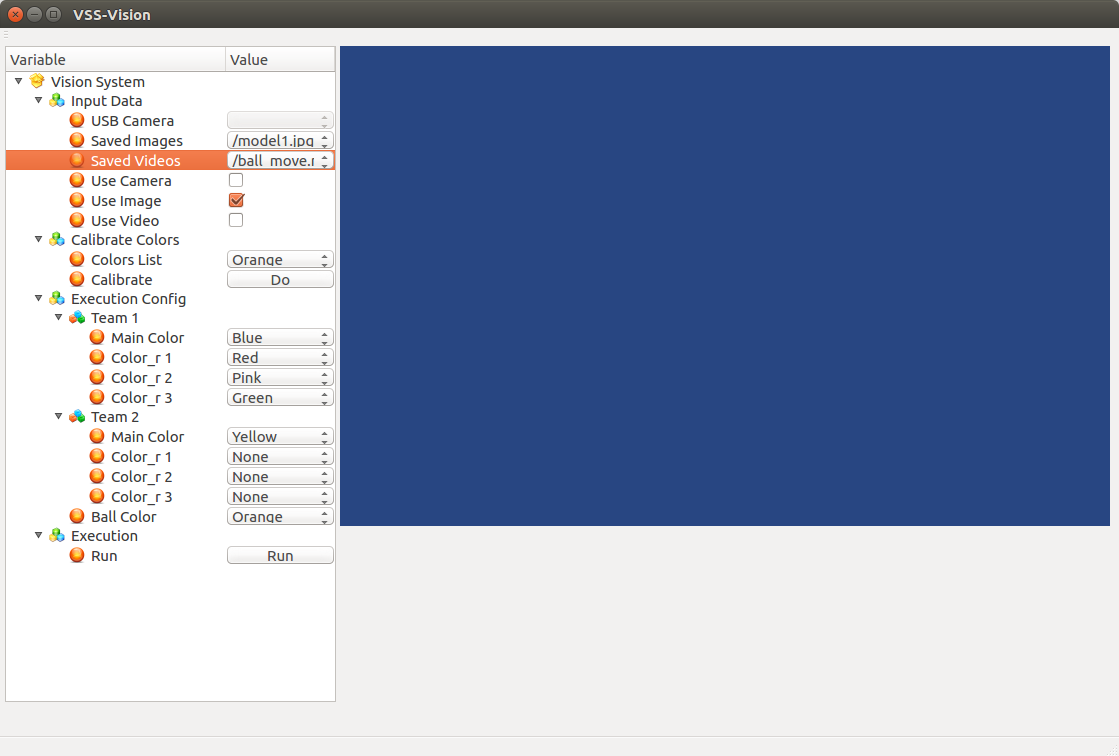
\includegraphics[width=0.5\textwidth]{vsssnovonormal.png} 	
	\caption{Nova interface do time da SIRLab \cite{VSSVision}}
	\label{SIRLabNova}
\end{figure}

O metodo de calibração de cores tambem foi modificado, segundo a equipe\cite{VSSVision} o sistema possibilita a calibragem de 8 cores, Laranja, Amarelo, Azul, Vermelho, Verde, Rosa, Roxo, Marrom. Após o usuário escolher uma cor para calibrar o mesmo deve encontrar um intervalo de cor, no espaço de cores HSV, que represente-a. Ao clicar na tela com o botão direito o sistema da um zoom na área para ajuste fino. A figura \ref{SIRLabNovaCalibracao} demonstra o novo metodo de calibração.

\begin{figure}[!h]
	\centering
	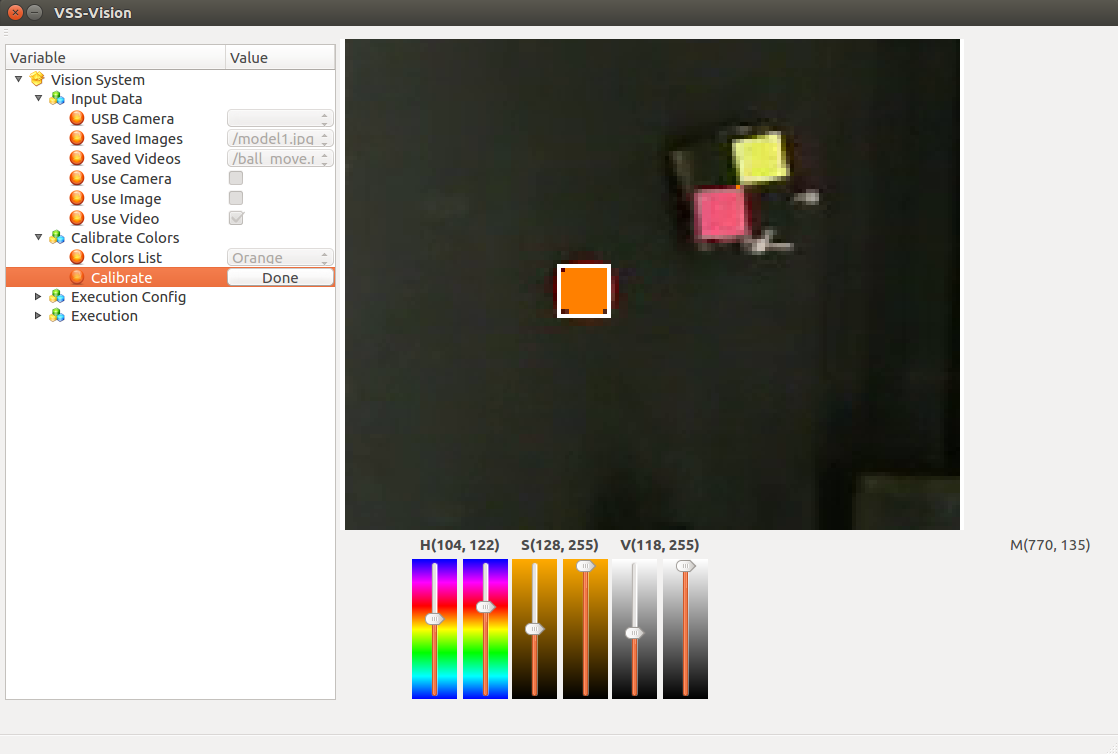
\includegraphics[width=0.5\textwidth]{vsssnovo.png} 	
	\caption{Calibração atual do time da SIRLab \cite{VSSVision}}
	\label{SIRLabNovaCalibracao}
\end{figure} % Fundamentação
	%====================================================================================================
	% ?????
	%====================================================================================================
	% TCC
	%----------------------------------------------------------------------------------------------------
	% Autor				: Jasane Schio
	% Orientador		: Gedson Faria
	% Co-Orientador		: Angelo Darcy
	% Instituição 		: UFMS - Universidade Federal do Mato Grosso do Sul
	% Departamento		: CPCX - Sistema de Informação
	%----------------------------------------------------------------------------------------------------
	% Data de criação	: 01 de Outubro de 2015
	%====================================================================================================
	
	\definecolor{dkgreen}{rgb}{0,0.6,0}
	\definecolor{gray}{rgb}{0.5,0.5,0.5}
	\definecolor{mauve}{rgb}{0.58,0,0.82}
	
	\lstset{frame=tb,
		language=C++,
		aboveskip=3mm,
		belowskip=3mm,
		showstringspaces=false,
		columns=flexible,
		basicstyle={\small\ttfamily},
		numbers=none,
		numberstyle=\tiny\color{gray},
		keywordstyle=\color{blue},
		commentstyle=\color{dkgreen},
		stringstyle=\color{mauve},
		breaklines=true,
		breakatwhitespace=true,
		tabsize=3
	}
	\chapter{Metodologia e Desenvolvimento} \label{Cap:Processamento}
	
			Para o desenvolvimento foi escolhida a biblioteca OpenCV por ser OpenSource, multiplataforma, conter uma grande quantidade de métodos e algoritmos já implementados	e pelo seu rápido desempenho de máquina.
			A linguagem escolhida para o desenvolvimento foi o C++ pois é uma linguagem de programação compilada, o que torna sua execução mais rápida que as linguagem interpretadas, dando ao sistema grande desempenho, e por ser uma linguagem orientada objeto. 
			
			O sistema desenvolvido é separado em duas partes: Processamento e Interface Gráfica.
			A parte de Processamento é onde são feitas as partes de aquisição de imagem, processamento de imagem, conversão de imagem para modelo de cor HSV, seleção de pontos de cor e contagem de ocorrência de cor. Já a interface gráfica, é a onde ocorre a entrada do usuário para assim ser feita a calibração manual de mínimos e máximos de cada cor.
		
	
	Passos do projeto:
	\begin{description}
		\item[Aquisição de imagens em vídeo:] Nesse passo as imagem são adquiridas via câmera USB.
		
		\item[Identificação de Objetos:]
				 Durante o processo de aquisição de imagem são selecionados os objetos, quais serão usados como base para a detecção de máximos e mínimos de cores.
		\item [Cálculo de Mínimos e Máximos:]
		 Nessa etapa são levados em consideração os objetos teste. A imagem é percorrida pixel a pixel na localidade dos objetos-teste e assim são salvos seus valores e feito a contagem de ocorrências de cada cor.		
	\end{description}


	\section{Projeto}
	\subsection{Organização do Projeto}
	 O projeto foi desenvolvido seguindo o paradigma de programação conhecido como  Orientação à Objetos, esse paradigma baseia-se na utilização de objetos individuais para criação de um sistema maior e complexo. A IDE usada para o desenvolvimento foi a QT Creator, esta separada o projeto em três pastas, Headers, Sources e Forms. Na pasta Headers estão os arquivos de cabeçalho(.h) onde estão as declarações dos métodos e variáveis usados nas classes  executáveis. Já na pasta Sources estão os arquivos fonte(.cpp), são nesses arquivos que os métodos declarados nos arquivos da pasta Header são implementados. Na pasta Forms está o arquivo de interface gráfica(.ui) que é usado no projeto para ser a ponte entre o usuario e as funções do sistema.
	 
	\begin{figure}[!h]
		\centering
		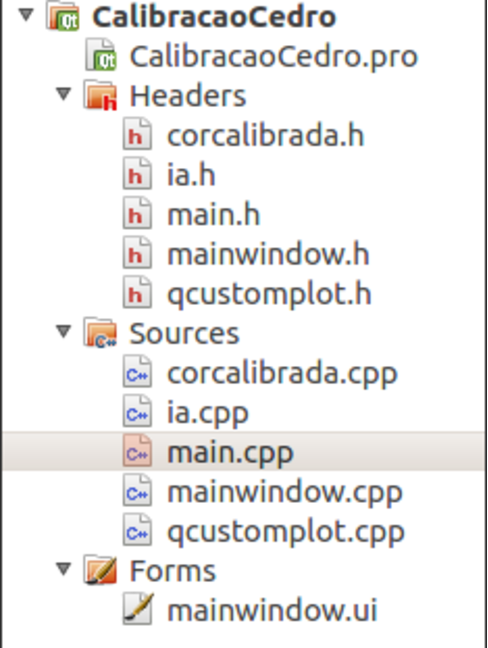
\includegraphics[width=0.2\textwidth]{organizacaoProjeto.pdf}
		\caption{Organização das pastas do projeto}
		\label{Organizacao do Projeto}
	\end{figure}
	Cada arquivo de cabeçalho possui um arquivo fonte correspondente, formando assim uma Classe, com exceção do arquivo fonte main, pois para este arquivo não há a necessidade.
	As classes desenvolvidas no projeto são:
 calibracao, manual, automatica, corcalibrada, janelaprincipal e tdestudent. Já a classe qcustomplot é um componente para auxilio em plotagem de gráficos e vizualização de dados\cite{QCustomPlot}.
Para melhor entendimento da interação entre as classes a figura 3.2 trás o diagrama de classes do projeto.
	 \begin{figure}[!h]
	 	\centering
	 	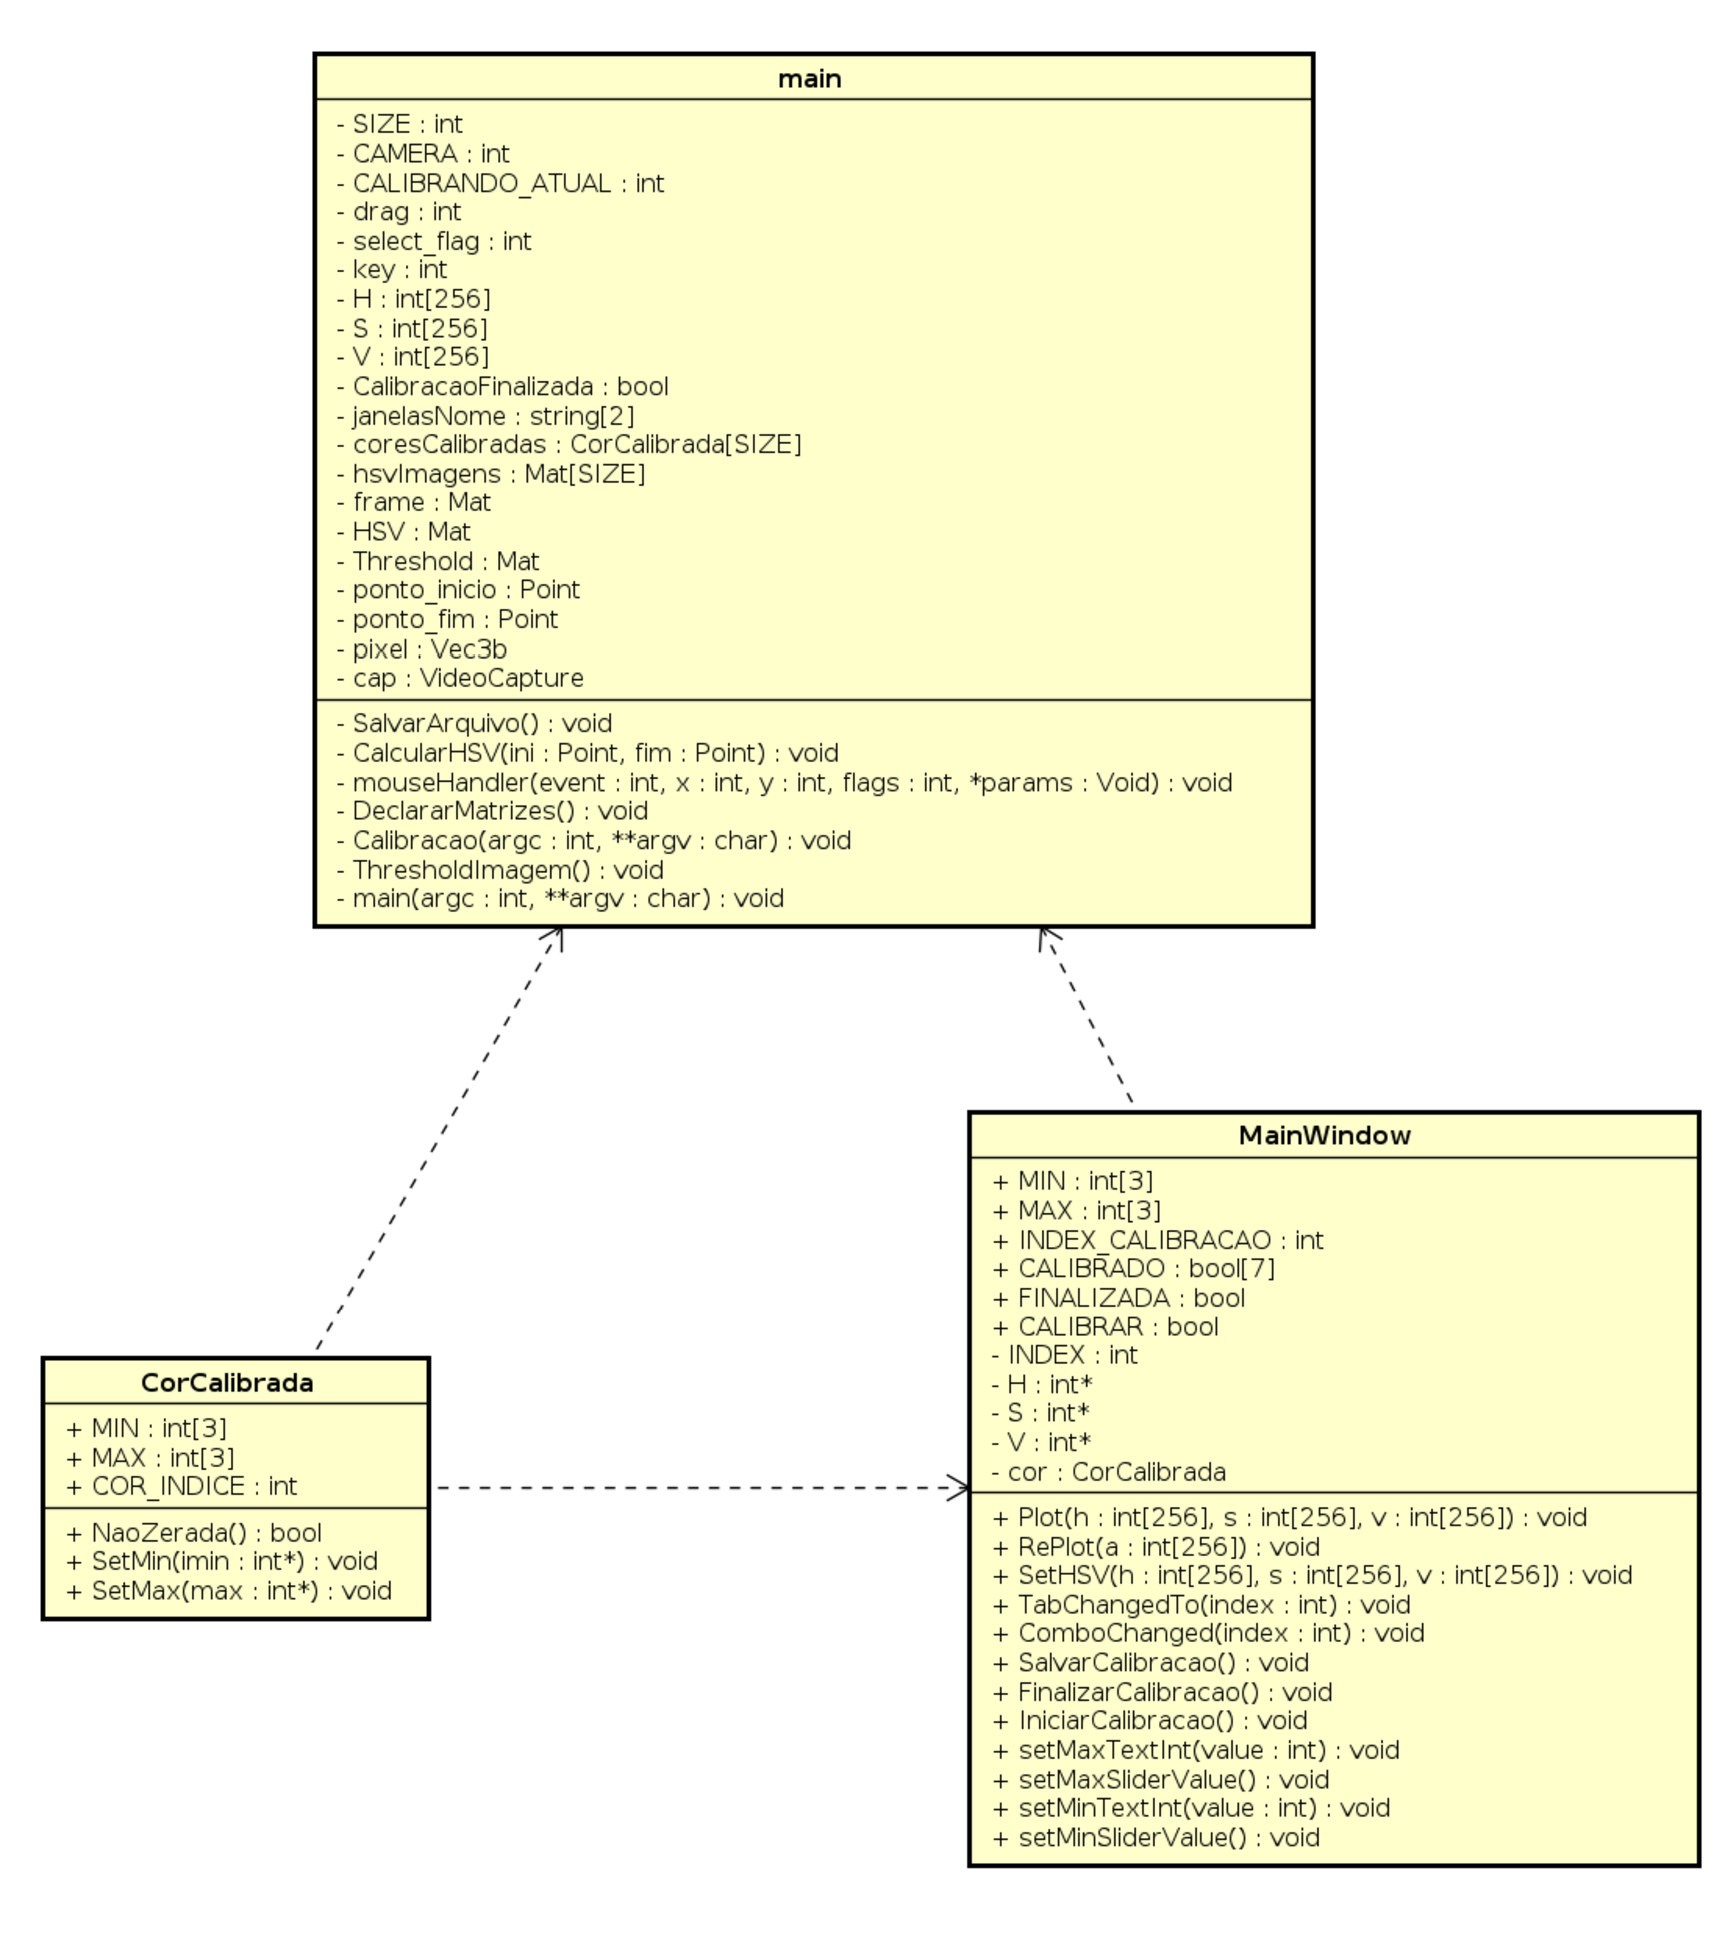
\includegraphics[width=0.8\textwidth]{diagramadeclasse.pdf}
	 	\caption{Diagrama de Classes do projeto}
	 	\label{DiagramaDeClasse}
	 \end{figure}\newpage


\subsection{Classes}
	\begin{description}

	\item [main] esta é a classe executavel do sistema, ela inicia o programa e em seguida chama a classe de interação grafica \textbf{janelaprincipal}  
	
	\item [janelaprincipal]	classe que faz a interação com o usuario e que de acorco com esta interação seleciona o tipo de calibração, e seus parametros, para então ser feita a analise dos pixeis	
		
	\item [calibracao] classe "pai" que contem os metodos e variaveis que virão a ser usadas por ambas as classes \textbf{manual} e \textbf{automatica}
	
	\item [manual] classe que contem os metodos, cálculo e variaveis necessarias para a calibração manual
	
	\item [automatica] classe que contem os metodos, cálculo e variaveis necessarias para a calibração automatica
			
	\item [corcalibrada] classe que salva o indice da cor já calibrada e seu intervalo de valores
	
	\item [tdestudent] esta é a classe que faz o cálculo probabilistico conhecido com TdeStudent
	

	\end{description}

	

	\section{O Sistema}

		\begin{figure}[!h]
			\centering
			\includegraphics[width=0.45\textwidth]{fluxoprincipal.pdf}
			\caption{Diagrama de Fluxo}
			\label{FlowCHart}
		\end{figure}
		A Figura 3.3 mostra o diagrama de fluxo do sistema, este com duas possibilidades: Calibração Manual e Calibração Automatica. Ambas são independentes uma da outra.  
		
		 O sistema consiste na apresentação da \textbf{interface gráfica} ao usuario. A \textbf{interface grafica} que por sua vez oferece as duas possibilidades ao usuario, de acordo com o tipo de calibração escolhido o sistema inicia a rotina de calibração referente. Apos a execução de toda o sistema é finalizada.
			
	\subsection{Calibração Automatica}	
		\begin{figure}[!h]
					\centering
					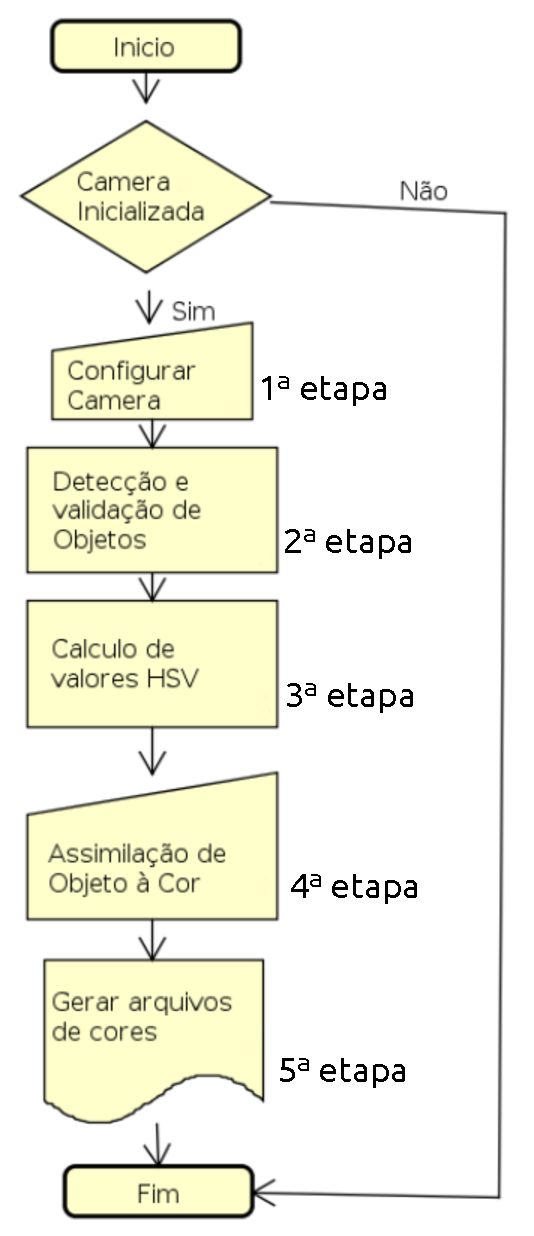
\includegraphics[width=0.45\textwidth]{fluxoautomatico.pdf}
					\caption{Diagrama de Fluxo Automatico}
					\label{DiagramaDeFluxoAutomatico}
				\end{figure} 
		Conformo mostrado na Figura \ref{DiagramaDeFluxoAutomatico} a rotina de calibração automatica possui cinco etapas. Este tipo de calibração  possui o mínimo possivel de interação com o usuario. O sistema faz automaticamente a detecção de objetos e utilizando a probabilidade matematica T de Student, considerando o tamanho de todos os objetos encontrados para encontrar os tamanhos minimo e maximo que os objetos desejados devem ter, nesse caso as etiquetas de cores dos robos, e só após determinar quais objetos possuem o tamanho desejado, analisar os valores e calcular as ocorrencias de cada um dos três valores do modelo HSV.
			
%	O fluxo inicia somente caso a camera esteja disponivel(1), apos a sua inicialização é feita a configuração da camera(2), enquadramento do tamanho correto e correção de brilho e luminosidade. Uma vez que a camera está configurada o sistema inicia a deteção de objetos e a validação dos objetos(3) que estão no tamanho correto. Apos deixar somente os objetos corretos no sistema, os pixeis de cada um são varridos e seu intervalo HSV encontrado(4). Os objetos e cores encontrados ficam disponiveis para o usuario apra esse fazer a assimilação entre os objetos e as cores corretas(5), após intervalos corretos já tiverem sido calibrados, um arquivo com os valores é gerado(6) e o usuario finaliza o sistema.
	
			
	Nas subsessões à seguir explicarei detalhadamente cada uma das etapas do processo de calibração automatica
	\subsubsection{1ª Etapa - Configuração de Camera}
Antes de ser feito a calibração propriamente dita são necessarias duas configurações: Ajuste de Constrate e Brilho e Recorte de Imagem.
A configuração de contraste e brilho utiliza o metodo \textit{convertTo} da biblioteca \textit{OpenCV} e é utilizada para o melhoramento da imagem antes da detecção dos objetos, a utilização completa fica da seguinte maneira:
\begin{center}
\centering \textit{ frameA.convertTo(frameA, -1, contrast\_value / 50.0, brightness\_value)}
\end{center}
Esta função recebe quatro parametros. O primeiro \textbf{frameA} informa aonde sera salvo o resultado da conversão. O segundo \textbf{-1} indica o tipo da matrix, ou numero de canais, da imagem a ser gerada, usa-se -1 quando se deseja que se use os valores semelhantes aos da imagem da imagem original\cite{OpenCV}, O terceiro \textbf{contrast\_value / 50.0} indica o valor de constraste, ou alpha, a ser usado para multiplicar os valores do pixel da imagem\cite{OpenCV} e por ultimo \textbf{brightness\_value} que é o valor do brilho, ou beta, a ser adicionado à imagem. \newline
Outra configuração feita é o Recorte de Imagem, onde utilizando a função setMouseCallback para possibilitar a interção do usuario na imagem por meio do mouse, sua utilização é dada da seguinte maneira:
\begin{center}
\centering \textit{ cv::setMouseCallback(src\_window,mouseHandler,0);}
\end{center}
Tem como primeiro parametro \textbf{src\_windows} que indica a janela na qual a função recebera a interação,  o segundo, \textbf{mouseHandler}, indica a função na qual esta implementada a interação e o ultimo parametro, \textbf{0}, indica parametros opcionais, neste caso não usaremos nenhum então foi usado o numero 0.
Dentro da função \textbf{mouseHandler} são identificados os pontos iniciai e final da seleção na tela e utilizada a função \textit{rectangle} para demarcar a seleção na tela. A utilização da função \textit{rectangle} completa fica da seguinte maneira:
\begin{center}
\centering \textit{ cv::rectangle(frameA, point1, point2, CV\_RGB(255, 0, 0), 2, 5, 0);}
\end{center}
A função rebece os parametros \textbf{frameA} indicando a imagem na qual será demarcada a area selecionada, depois o parametro \textbf{point1} que é o ponto incial de seleção na imagem, \textbf{point2} que é o ponto final da seleção. \textbf{CV\_RGB(255, 0, 0)} que indica a cor da demarcação, \textbf{2} indicando a expessura da demarcação, \textbf{5} que significa o tipo de linha a ser utilizado na demarcação e \textbf{0} que é o numero de bits fracinarios.
 Após confirmada a escolha do tamanho da tela 
este é então salvo na variavel nomeada \textit{tamanho}, está então sera usado durante todo o processo de calibração.
\newpage
\subsubsection{2ª Etapa - Detecção e validação de Objetos}
A detecção dos objetos a serem calibrados é dada pelo algoritmo de detecção de bordas de Canny. Como mais um recurso para eliminação de ruidos e melhoria da imagem antes de ser executado a detecção de objetos atravez da detecção de bordas é utilizado desfoque na imagem. O algoritmo de Canny já está implementado dentro da biblioteca OpenCV e com a seguite usagem:
\begin{center}
\centering \textit{  Canny(src\_gray, canny\_output, thresh, thresh * 3, 3);}
\end{center}
O algoritmo de Canny utiliza por padrão imagem em padrões de cinza, sendo assim \textbf{src\_gray} é a imagem orignal tranformada para escala de cinza, esta é a imagem na qual o algoritmo sera aplicado. \textbf{canny\_output} será a imagem de saida da função.
\textbf{thresh} e \textbf{thresh*3} são os limites mínimos e máximos para considerar uma borda. \textbf{3} é o valor de apertura ou kernel, o valor 3 é utilizado como padro.

Apos o uso do algoritmo de Canny para detecção de bordas é necessario então fazer uso da função \textit{findContours}, nativa no \textit{OpenCV} para detecção de contornos.
\begin{center}
\centering \textit{ findContours(canny\_output, contours, hierarchy, CV\_RETR\_EXTERNAL, CV\_CHAIN\_APPROX\_SIMPLE, Point(0, 0))}
\end{center}

O primeiro parametro, \textbf{canny\_output}, é a imagem que o algoritmo de Canny gerou com as bordas encontrada na imagem, e é a imagem que o método \textit{findContours} ira utilizar para detectar os contornos, \textbf{contours} é o parametro que indica onde serão salvos os contornos encontrados, cada contorno é armazenado como sendo um vetor de pontos \cite{OpenCV}. \textbf{hierarchy} é onde será salva um verot de informações sobre a topologia da imagem, e terá como total de elementos o mesmo numero que o total de contornos encontrado\cite{OpenCV}. O quarto parametro, \textbf{CV\_RETR\_EXTERNAL} indica o modo de obtenção de contornos, nesse caso \textit{CV\_RETR\_EXTERNAL} indica que o metodo só obtera os contornos exteriores\cite{OpenCV}. \textbf{CV\_CHAIN\_APPROX\_SIMPLE} indica o metodo que sera usado para aproximação de contornos, o metodo \textit{CV\_CHAIN\_APPROX\_SIMPLE} comprime segmentos horizontais, verticais, diagonais e deixa apenas os seus pontos finais\cite{OpenCV}. E o ultimo parametro, \textbf{Point(0, 0)}, indica o valor a ser usado para deslocar a imagem ao encontrar os objetos, neste caso esse valor é 0 para Y e 0 para X, pois não sera necessario. 

Uma vez obtidos os contornos é necessarios que se faça a eliminação de vertices dos polignos encontrados nos objetos deixando assim o objeto mais preciso. Isso é necessario para deixar a forma encontrada mais precisa dá forma original. Para este ajuste foi usado o metodo \textit{approxPolyDP}, ja implementado dentro da biblioteca OpenCV. Esse metodo teve que ser aplicado em cada um dos contornos encontrados, e foi utilizado da seguinte maneira:
\begin{center}
\centering \textit{    approxPolyDP(Mat(contours[i]), contours\_poly[i], 3, true)}
\end{center}
 Onde o metodo inicia recebendo como paralametro, \textbf{Mat(contours[i])} que é a criação de uma nova imagem, somente com aquele unico objeto, que esta sendo analisado. A seguir é informado no segundo parametro a variavel de destino \textbf{contours\_poly[i]}, onde sera salvo o objeto com a eliminação dos vertices. O terceiro parametro indica o valor do \textit{epilson}, usado o valor \textbf{3} que especifica a precisão da aproximação, a distância máxima entre a curva original e a sua aproximação\cite{OpenCV}. O ultimo parametro indica se a curva aparoximada sera fechada ou não, foi usado o valor \textbf{true} pois neste caso fechar um uma curva é necessario para que o objeto onde está a cor, seja idenficado e analisado na probabilidade.
 
 Por ultimo os objetos possuem sua borda ignorada, sendo assim calculado o tamanho interior dele, para que por ventura não hajam pixeis de cor preta ou derivadas a serem calculadas.
 
 A detecção de contorno detecta todos os contornos possiveis na imagem, isso inclue sombras, luzes entre outras coisas. Mas não são todos os objetos encontrados que deverão ser calculados, sendo assim foi usado o cálculo probabilistico T de Student.
 Foi implementado uma biblioteca para o uso da probabilidade voltada para objetos Rect, os objetos da biblioteca \textbf{OpenCV} obtidos na detecção. Essa biblioteca analisa a lista de objetos encontrados na detecção e faz o cálculo dos limites, tamanho mínimo e máximo, dos objetos. Apos a obtenção desse limite pela biblioteca são analisados todos os objetos encontrados na detecção e os cujo tamanho não esteja dentro deste limite são removidos da lista.
 
 \subsubsection{3ª Etapa - Calculo de valores HSV}
 Para que possam ser feitos os cálculo de valores HSV mínimo e máximos é necessario que se faça, primeiramente a conversão da imagem obtida pela camera, normalmente no espaço de cores RGB, para o espaço de cores HSV, pois a mesma lida melhor com deferenças de luminosidade. 
 A biblioteca \textbf{OpenCV} converte o espaço de cor usando a função \textit{cvtColor} que utiliza da imagem original, e de uma imagem vazia com memoria alocada para ser salva a imagem apos a conversão, além do parametro do tipo de conversão, Exemplo do uso do método:
\begin{center}
\centering \textit{cvtColor(frame, HSV, CV\_RGB2HSV);}
\end{center}

Apos a conversão é necessario, então, ser feita uma analise dos objetos encontrados. Para cada objeto serão somadas as ocorrencias de cada um dos valores, HSV, e salvos separadamente em um vetor para cada, H, S e V com 256 posiçoes, uma vez que se sabe que os valores de um pixel varial de 0 a 255. As ocorrençias são salvas se baseando no valor HSV do pixel. Para isso o pixel é separado em valores H, S e V este então tera seu valor correspondente a posição no vetor apropiado, por exemplo, se o valor de H em um determinado pixel for de 87, a posição de numero 87 no vetor ganhara uma ocorrencia a mais. No codigo, fica da seguinte maneira:
	        
	        \begin{algorithm}
	       		 \caption{Contagem dos Valores HSV}
		        \begin{algorithmic}
		     	
		     	\ForAll{objeto encontrado} 
		   		 \State ValoresH[objeto.valorh]++ 
		    	 \State	ValoresS[objeto.valors]++ 
		     	 \State	ValoresV[objeto.valorv]++
		     	\EndFor
		     		
		        \end{algorithmic}
	        
	        \end{algorithm}
	        
        
Uma vez terminada a analise dos pixeis do objeto o sistema procupa o valor mínimo e máximo, ou seja a primeira e ultima ocorrencia. Esses valores são encontrados procurando o primeiro valor de pixel que não esta zerado e o ultimo valor que não esta zerado. Isto é feito para eliminar que durante a analise o numero de valores a serem comparados ao valor real do pixel, da imagem final, seja menor. Para exemplificar a Figura 3.6 tras o gráfico dos valores de H da calibração de um certo objeto antes de ser feia a eliminação dos valores. Se fosse analisado esses valores, não eliminando os valores zerados, o sistema buscaria no valor de H do pixel desde o valor 1 ao 126 sem a necessidade, pois se não houve ocorrencia desses valores no objeto de referencia, o que foi analisado, então esses valores não fazem parte da cor desejada.
% e tambem para remover ruidos de outros cores para que estas não interfiram na pureza da busca da dada cor.

\begin{figure}[!h]
	\centering
	\includegraphics[width=0.5\textwidth]{graficototal.png}
	\caption{Grafico Exemplificando a Ocorrencia dos valores de H.}
	\label{Grafico Exemplo}
\end{figure}

 Apos ser feita a eliminação, Figura 3.7, de valos sabemos que somente a partir do pixel 110 houve ocorrencia, assim quando for necessario analisar pixel a pixel, os valores abaixo de 110 serão ignorados, ou seja não fazem parte da cor desejada.
 \begin{figure}[!h]
 	\centering
 	\includegraphics[width=0.5\textwidth]{graficominmax.png}
 	\caption{Grafico Exemplificando a Ocorrencia dos valores de H após eliminação.}
 	\label{Grafico Exemplo}
 \end{figure}

Após serem encontrados os valores mínimo e máximos para H, S e V de cada objeto detectado, estes valores são salvos em uma lista de objetos do tipo CorCalibrada. Neste objeto são salvos os respectivos valores.

 \subsubsection{4ª Etapa - Assimilação de Objeto à Cor}
 Uma vez que os objetos já foram identificados, suas cores analisadas e gerada sua lista. O sistema, utilizando do recurso de interface gráfica disponivel pela biblioteca Qt, informa ao usuario uma lista com os intervalos de cores encontrados, e outra lista com as possiveis cores a serem assimiladas para eles. Assim o usuario pode analisar um por um dos objetos e escolher qual se assemelha a qual cor. Assim que assimilada a cor ao objeto este é salvo e seu objeto CorCalibrada na lista de objetos salva o valor da cor em seu atributo COR\_INDICE.
 
  \subsubsection{5ª Etapa - Gerar Arquivo de Cores}
  Assim que todas as cores já estiverem sido assimiladas e a calibração finalizada, gera-se um arquivo chamado \textbf{cores.arff} contendo o indice de cada cor calibraa e seus valores máximos e mínimos.
  
  		
  	\subsection{Calibração Manual}
  	
  	  		\begin{figure}[!h]
  	  				\centering
  	  				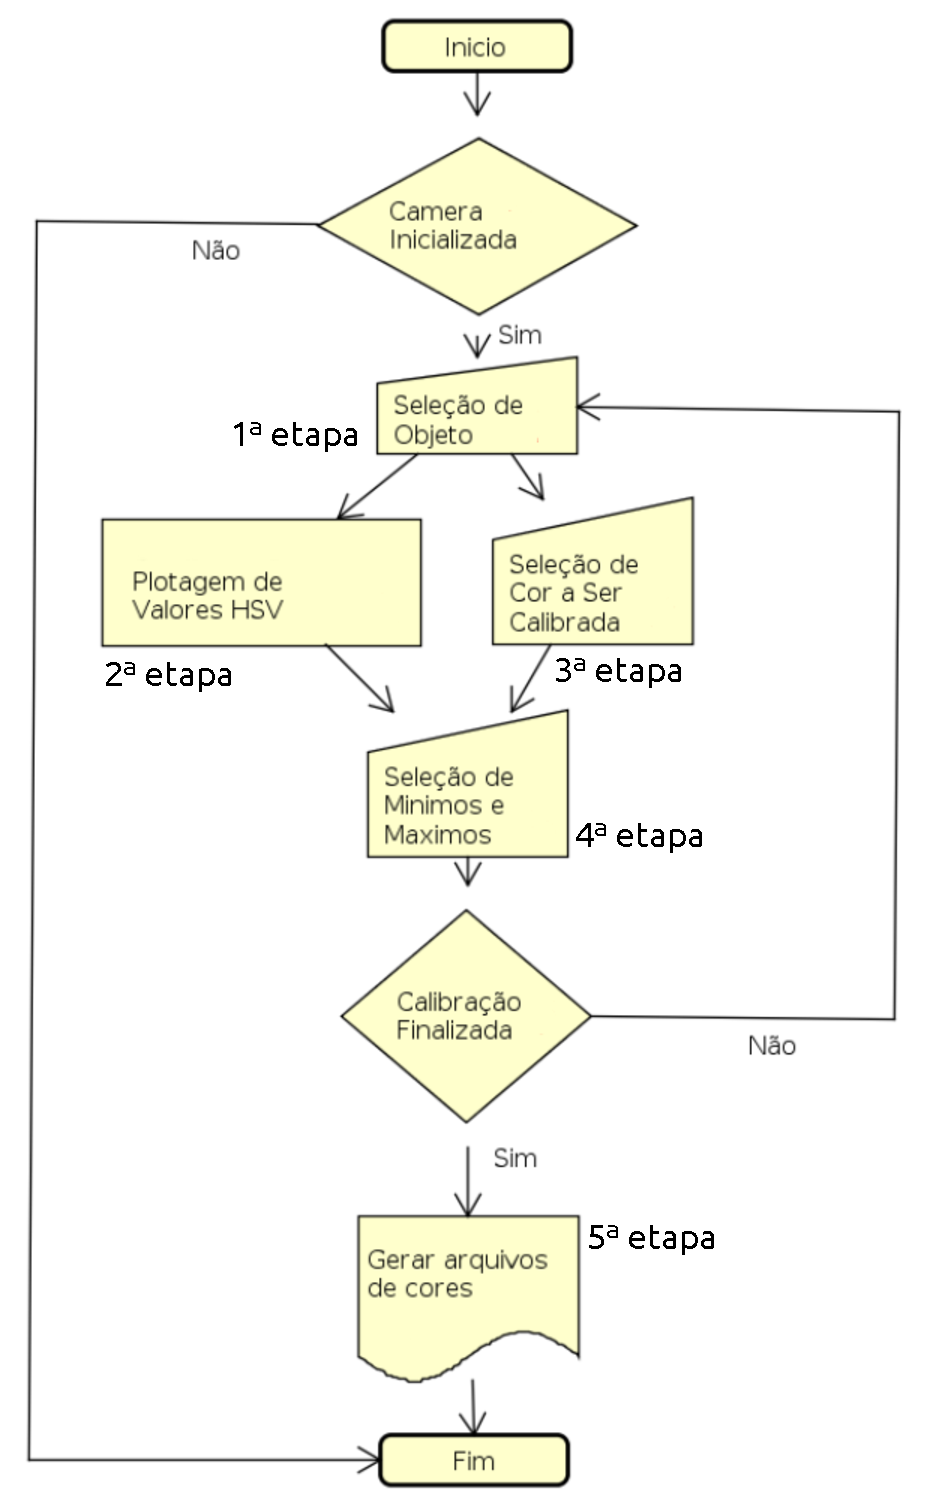
\includegraphics[width=0.45\textwidth]{fluxomanual.pdf}
  	  				\caption{Diagrama de Fluxo Manual}
  	  				\label{DiagramaDeFluxoManual}
  	  			\end{figure}
  	  		
  	  			
   A Figura \ref{DiagramaDeFluxoManual} mostra o fluxo de calibração manual, o sistema possui cinco etapas que permanecem em repetição até que todos os objetos sejam calibrados. Como o próprio nome já indica, o metodo de calibração é manual, sendo assim é necessario que o usuario selecione o objeto que o mesmo quer calibrar.
%   Após a camera ser inicializada(1) o sistema espera pela seleção do objeto(2) o qual tera seus pixeis calculados para gerar os valores HSV. Com o objeto selecionado o usuario escolhe então a cor(4), na opção de escolha de cor, e calibrar. A area selecionada é então analisada e os valores de cada pixel calculados analisando seu HSV(3).
%   	O usuario então seleciona os valores que considera satisfatorios(5). Enquanto houverem objetos a serem calibrados(6) o sistema repete esta mesma rotina, quando todos os objetos já tiverem sido calibrados, um arquivo com os valores é gerado(7) e o usuario finaliza o sistema.
	
  	\subsubsection{1ª Etapa - Seleção de Objeto}	
  	O primeiro passo para ser feita a calibração manual é a seleção de Objeto. Com o auxilio da função setMouseCallback, disponivel na biblioteca \textbf{OpenCV} e já explanada na sessão 3.2.1, é possivel obter os pontos de uma seleção feita na imagem, seu uso é necessario, já que obtenção de um ou mais objetos com a \textbf{mesma cor} a serem analisados é feita somente com a interação do usuario. Neste seleção existe a possibilidade de escolher somente um objeto ou mais de um objeto da mesma cor em diferentes pontos do campo, a seleção é feita somente um objeto por vez e cada objeto é analisado e seu valor e ocorrencia calculado utilizando o mesmo metodo encontrado na sessão 3.2.1 subsessão \textbf{Calculo de valores HSV}, estes valores são armazenados em memoria de execução e somente mostrados ao usuario quando requisitados. 
  	
  	\subsubsection{2ª Etapa - Plotagem de Valores HSV}	
  	Uma vez que o usuario já selecionou todos os objetos e os mesmos já foram analisados, o processo de calibração encaminha à interface grafica os valores encontrados e está plota três gráficos, um para cada um dos valores HSV.
  	Com a ajuda do componente auxiliar qcustomplot os gráficos são mostrados no sistema informando para o usuario quais foram os valores obtidos na seleção.
  	
  	\subsubsection{3ª Etapa - Seleção de Cor a ser Calibrada}
  	A seleção da cor na lista de cores possiveis para ser assimilado, pode ser considerada uma ação concomitante à ação de plotagem de graficos sendo que uma não depende dá outra, já que no momento da seleção do objeto o usuario já tinha em mente qual era sua cor, e a plotagem do gráfico não interfere nessa escolha, já a plotagem do gráfico é uma ação somente visual e não tem influencia da cor escolhida.
  	
  	\subsubsection{4ª Etapa - Seleção de Minimos e Maximos}
  	 Assim que os graficos são plotados, se torna então possivel, utilizando o recurso Slider, de fazer a seleção dos valores, tanto mínimo, quanto máximo. Ao ser modificado, cada um dos valores, o gráfico se ajusta para melhor detalhar ao usuario a ocorrencia dos pixeis. Ao contrario do sistema automatico, no sistema manual o objeto CorCalibrada só é criado após a seleção da cor e dos intervalos pelo usuario. Quando este salva a cor na interface gráfica, a mesma cor é encaminhada para o sistema manual e assim salva na lista.
  	 
  	 
\subsubsection{5ª Etapa - Gerar Arquivo de Cores}
Do mesmo modo que ocorre na calibração automatica, uma vez que todas as cores já estiverem sido assimiladas pelo usuario, este então finaliza a calibração e um arquivo com os valores calibrados é salvo localmente.
  	   	
  		
  	
%\include{aplicativo} % Aplicação
%\include{resultados} % Resultados
%\include{conclusao} % Conclusão

\cleardoublepage
\phantomsection
\addcontentsline{toc}{chapter}{Referências Bibliográficas}
%\bibliographystyle{abnt}
%\bibliographystyle{abnt-num} % Numérico
\bibliographystyle{abntex2-num} % Autor-Data
%\bibliographystyle{abbrv}
%\bibliographystyle{apalike} 
%\bibliographystyle{ieeetr} % Ordena por ordem de aparição.  
<<<<<<< HEAD
\bibliographystyle{abntex2-num} % Ordena por ordem alfabetica com nomes abreviados.
=======
%\bibliographystyle{abbr} % Ordena por ordem alfabetica com nomes abreviados.
>>>>>>> CoderSquirrel/master
%\bibliographystyle{plain} % Ordena por ordem alfabetica com nomes por extenso.
\bibliography{bibliografia.bib} % commented if *.bbl file included.


\addcontentsline{toc}{chapter}{Ap\^endices}
\appendix
%\include{apendice}

\end{document}
